\documentclass[10pt,a4paper]{article}
\usepackage[utf8]{inputenc}
\usepackage{amsmath}
\usepackage{amsfonts}
\usepackage{amssymb}
\usepackage{graphicx}
\usepackage{amssymb}
\usepackage{hyperref}
\author{Stanley Akor}
\title{Physical Problem Solving}
\begin{document}
\maketitle
\newpage
\section*{Question 1}
\begin{figure}[h!]\label{d1}
\centering
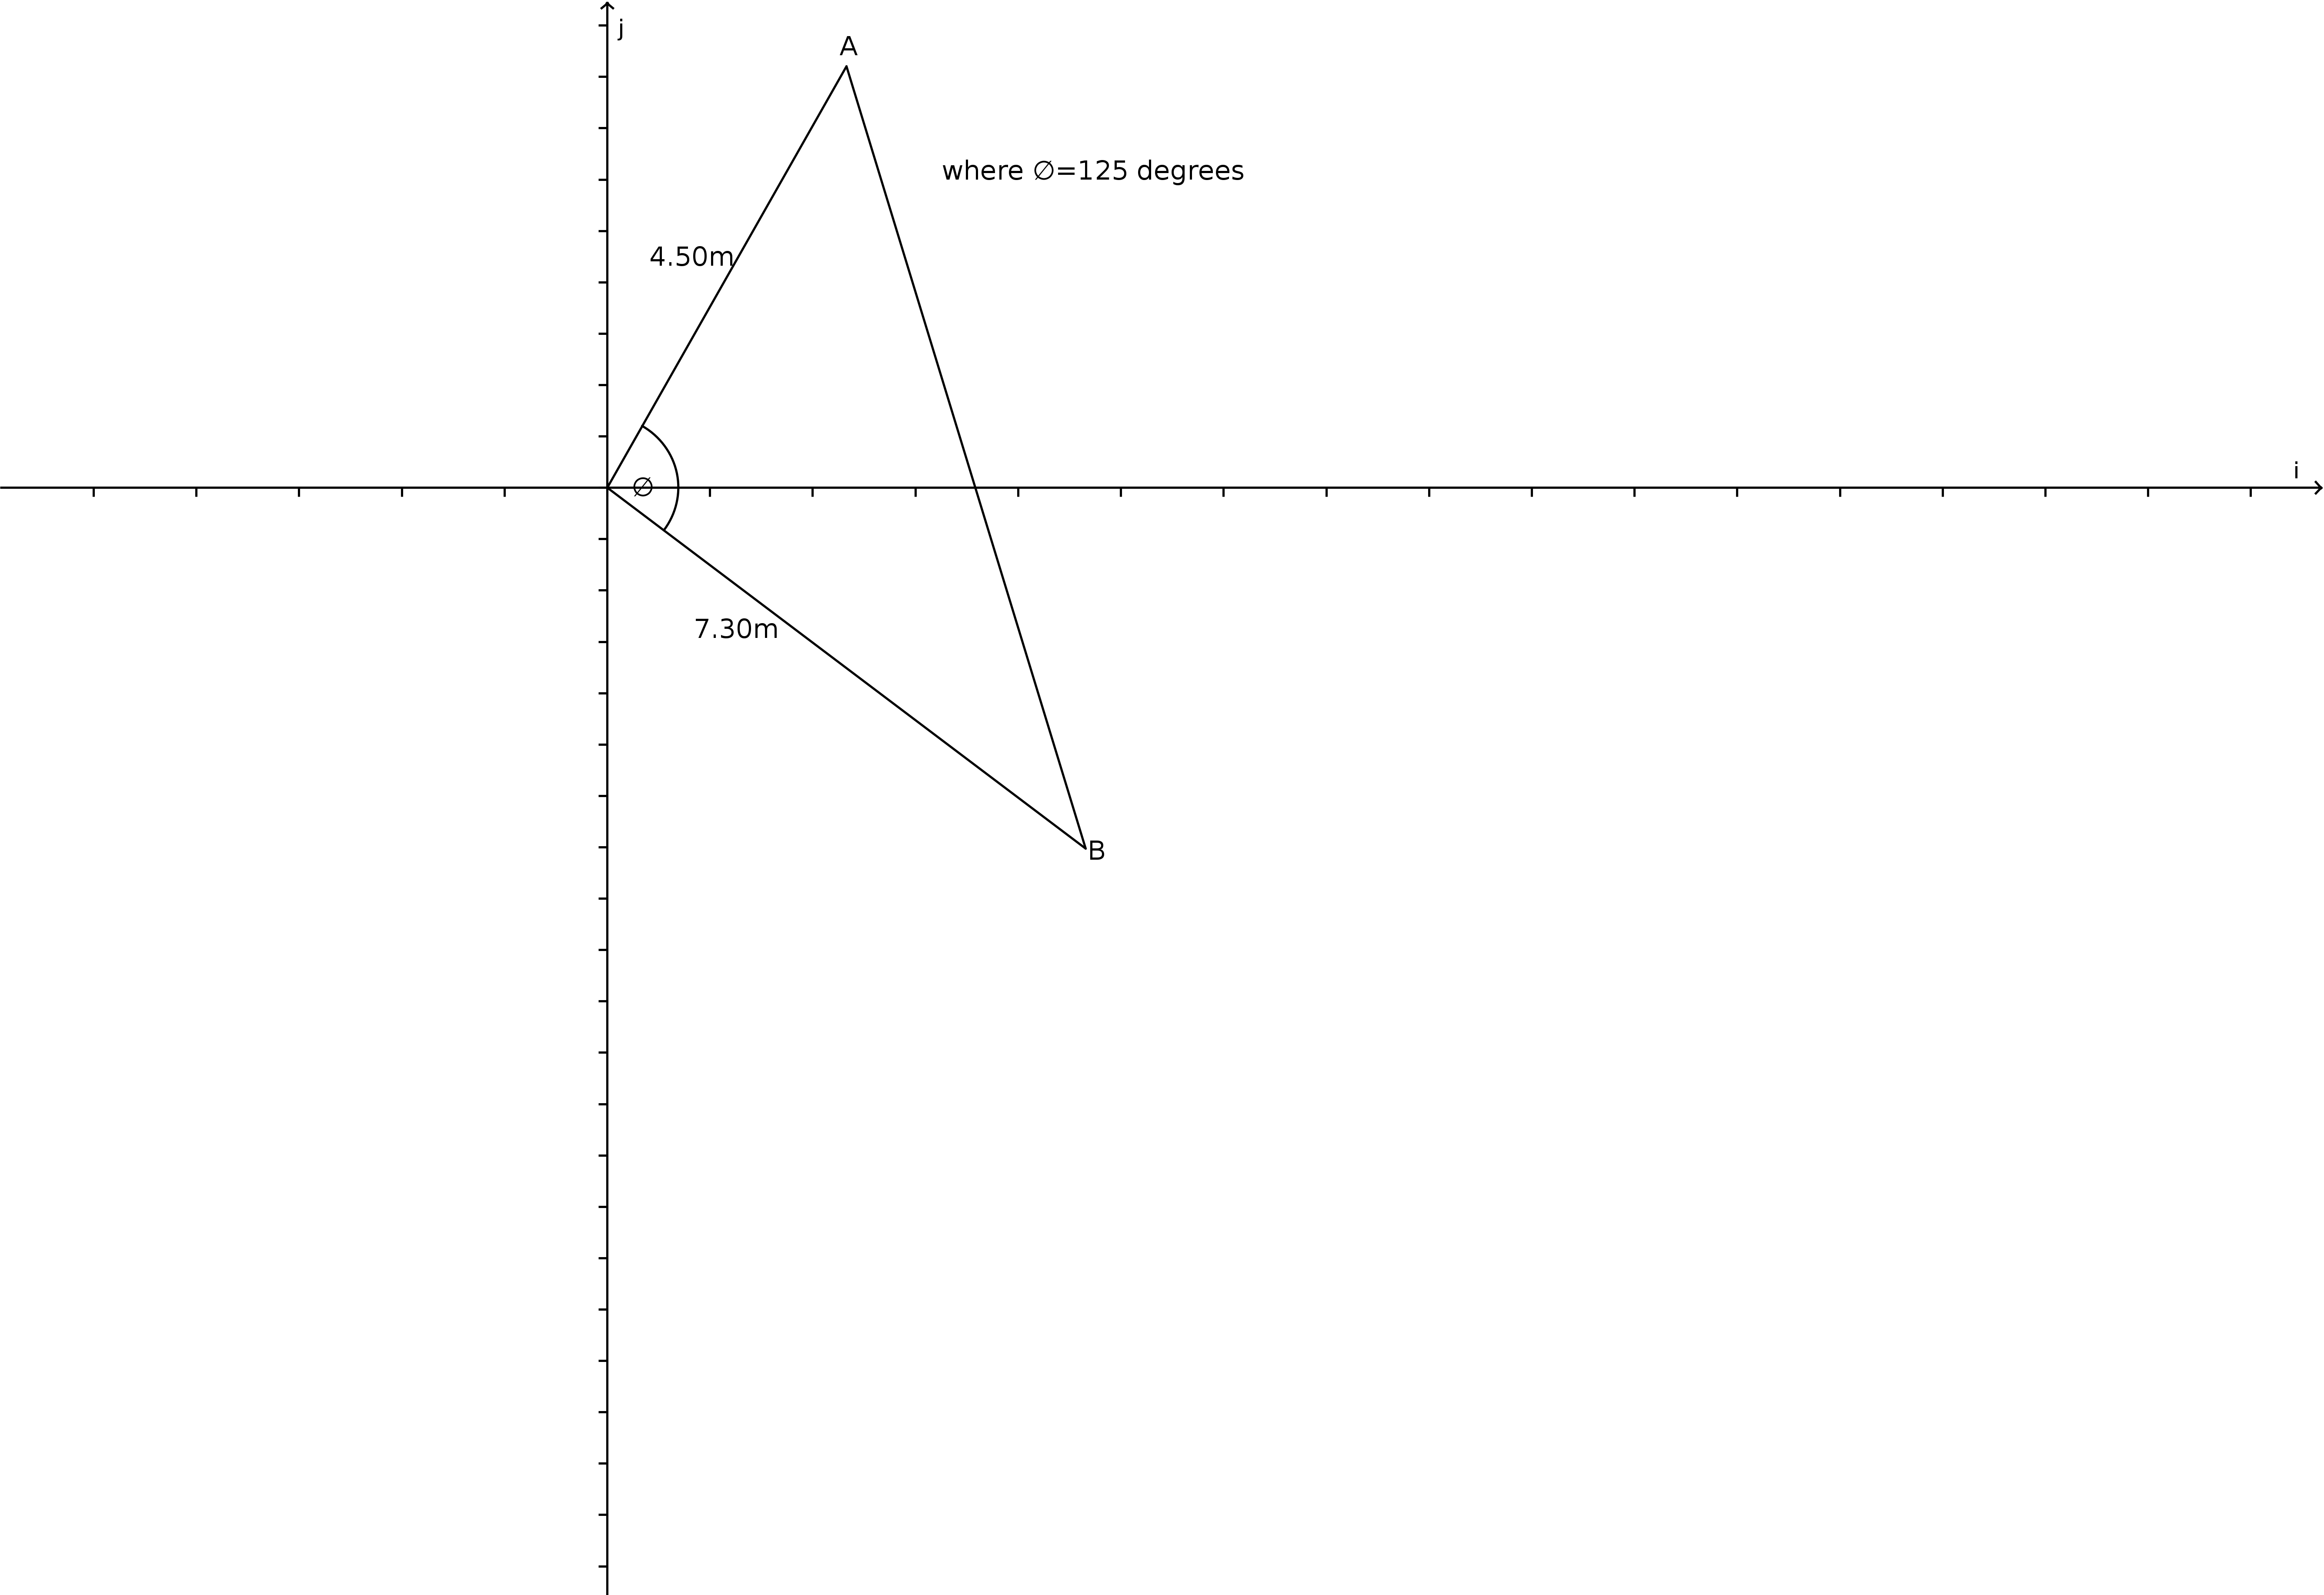
\includegraphics[scale=0.3]{qsn1.png}
\caption{Vector Diagram}
\end{figure}
\begin{itemize}
\item[a] $\overrightarrow{A}\centerdot\overrightarrow{B}$\\
The scalar product of the vectors is obtained by multiplying the magnitude of the vectors by the cosine of their angle.

$$\overrightarrow{A}\centerdot\overrightarrow{B}
=|\overrightarrow{A}|\overrightarrow{B}|\cos\theta$$

$$\overrightarrow{A}\centerdot\overrightarrow{B}=4.50\times7.30\cos\left(125^\circ\right)$$
$$\therefore \overrightarrow{A}\centerdot\overrightarrow{B}= -18.84$$

\item[b]$\overrightarrow{A}\times\overrightarrow{B}$\\
Observe that the two vectors$\overrightarrow{A}$ and $\overrightarrow{B}$ have both $i$ and $j$ components, so we have to resolve these vectors both horzontally and vertically,we can write the vectors component-wise as;\\

$$\overrightarrow{A}=|\overrightarrow{A}|\cos\left(40^\circ\right)\hat{i}-|\overrightarrow{A}|\sin\left(40^\circ\right)\hat{j}$$\\
$$\overrightarrow{B}=|\overrightarrow{B}|\cos\left(85^\circ\right)\hat{i}+|\overrightarrow{B}|\sin\left(85^\circ\right)\hat{j}$$
We can now find the cross product of these two vectors by computing their determinant.

\begin{equation}
\begin{vmatrix}
\hat{i}& \hat{j} & \hat{k} \\ 
|\overrightarrow{A}|\cos\left(40^\circ\right) & -|\overrightarrow{A}|\sin\left(40^\circ\right) & 0\\ 
|\overrightarrow{B}|\cos\left(85^\circ\right) & |\overrightarrow{B}|\sin\left(85^\circ\right) & 0 
\end{vmatrix} 
\end{equation}
$\therefore \overrightarrow{A}\times\overrightarrow{B}=\left(|\overrightarrow{A}||\overrightarrow{B}|\sin\left(85^\circ\right)\cos\left(40^\circ\right)+|\overrightarrow{A}||\overrightarrow{B}|\cos\left(85^\circ\right)\sin\left(40^\circ\right)\right)\hat{k}$\\
$$\overrightarrow{A}\times\overrightarrow{B}=|\overrightarrow{A}||\overrightarrow{B}|\sin\left(85^\circ+40^\circ\right)\hat{k}$$\\
$$\overrightarrow{A}\times\overrightarrow{B}=4.50\times7.30\sin\left(125^\circ\right)\hat{k}=26.90\hat{k}$$
We therefore conclude that the cross product of vector $A$ and $B$ produces a vector with magnitude 26.90 in the $\hat{k}$-direction.

\end{itemize}
\section*{Question 2}
From the pieces of information given in the question,we have that;
The horizontal distance between the boy and the middle of the basket is $D$,$D$ can also be refered to as the range of the projectile motion, the angle of inclination is $55^\circ$,substituting these values into our range equation for the projectile motion,we shall obtain the initial velocity of the ball.

$$Range=\frac{U^2\sin2\theta}{g}$$
where $\theta=55^\circ$, Range=4.20m and g=9.8$ms^{-2}$\\
$$U=\left(\frac{9.8\times4.2}{\sin\left(110^\circ\right)}\right)^{\frac{1}{2}}$$
$$U=6.618ms^{-1}$$

\newpage
\section*{Question 3}
\begin{figure}[h!]\label{d1}
\centering
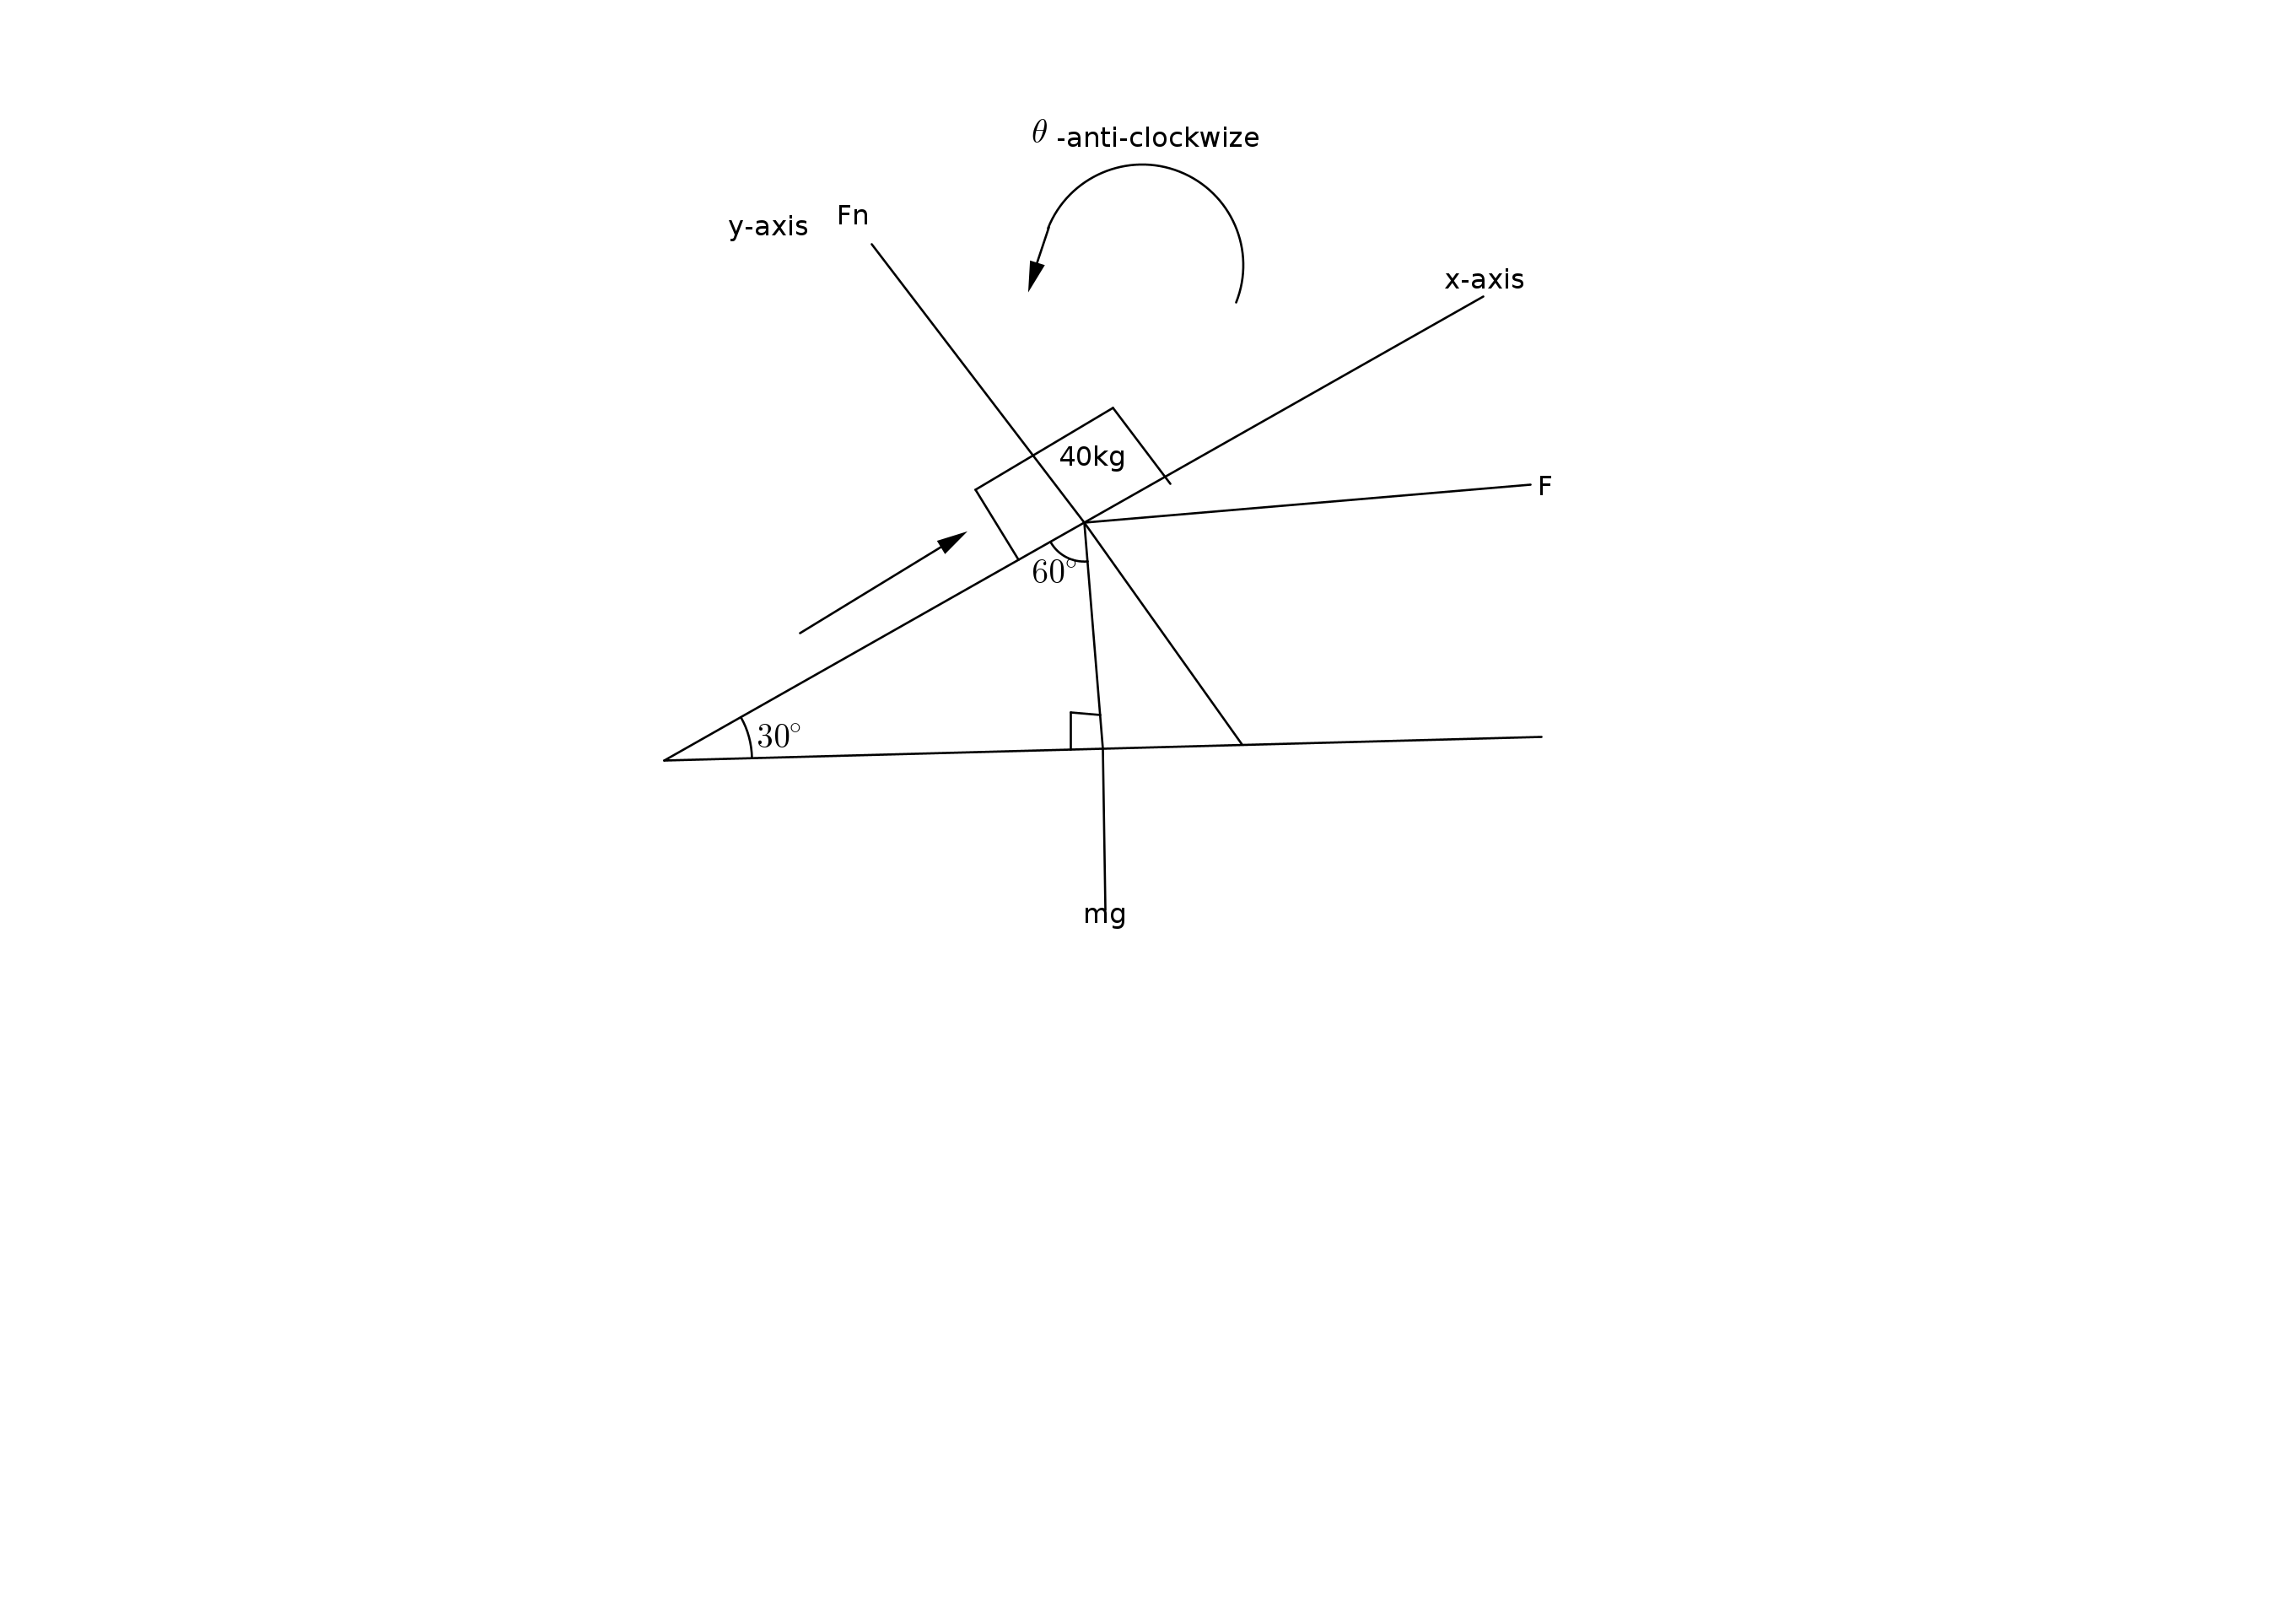
\includegraphics[scale=0.5]{ttt.png}
\caption{Force Diagram}
\end{figure}
Considering the force diagram of the box moving along an inclined plane as shown above, we can resolve the forces into their respective $x$ and $y$ components

\begin{table}[h!]
\centering
\begin{tabular}{c c c}
Force & x-components & y-components\\
$\overrightarrow{Fn}$& Fncos90 & Fnsin90\\
mg& mgcos(240)&mgsin(240)\\
$\overrightarrow{F}$ & Fcos(330)&Fsin(330)
\end{tabular}
\end{table}
Now let's resolve the forces to their respective components,starting with the x-component $R_{x}$.\\
$$R_{x}=Fncos90+mgcos240+Fcos330=ma$$
Since the body is moving at a constant speed, acceleration $a=0$, so that the right hand part of the equation turns to zero. 
$$R_{x}=Fncos90+mgcos240+Fcos330=0$$
Where m=40kg and g=9.8m$s^{-2}$
$$R_{x}=0-196+0.866F=0$$
$$F=\frac{-196}{-0.866}=226.32N$$
Therefore the force required to sustain the motion is 226.32N.\\
Now let's consider the y-axis, we take as similar approach as we did for the x-axis.
$$R_{y}=Fnsin90+mgsin240+Fsin330=ma.$$
$Acceleration=0$, $F=226.32N$, $ma=0, sin90=1,m=40kg,g=9.8ms^{-1}$.
$$ Fn-339.481-(226.32)(-0.5)=0$$
$$\therefore Fn=451.641N$$
The force exerted on the ramp by the crate is $451.641N$. 
\end{document}